\documentclass[UTF8,a4paper]{article}% 文档格式
\usepackage{graphicx}
\usepackage{physics}
\usepackage{ctex}
\usepackage{times}% 英文使用Times New Roman
\usepackage[left=1cm,right=1cm,top=1.80cm,bottom=1.8cm]{geometry}
\usepackage{fancyhdr}
\pagestyle{fancy}
\usepackage{multirow} %Table Support
\usepackage{siunitx}
\usepackage{float}

\title{\textbf{基础物理实验报告\\功函数}}
\author{杨哲涵~~~工物22班~~~2022011105}
\date{2023年10月20日}
\begin{document}
\maketitle
\lhead{2023年基础物理学实验A2}
\chead{}
\rhead{42a}
\lfoot{}
\cfoot{\thepage}% 页脚中间显示页码
\rfoot{}
\section*{摘要}
电子逸出金属表面需要获得一定的能量,例如,真空玻璃管中的电极通过电流加热后,能够向另一端发射电子,这份能量与电子的功函数有关.本实验采用里查孙直线法,通过多次改变阴极温度与加速电压,测量真空管阴极材料钨的电子功函数,了解热电子发射的规律.
\section{实验原理与仪器}
逸出功(aka.功函数)定义为「无穷远处真空中一静止电子与物质内部费米能级上一电子之间的能量差」.认为金属与真空的边界上存在一个大于$E_f$($T=0\unit{\kelvin}$时电子的最大能量)的势垒$W_a$,那么$\Phi=W_a-E_f$就是功函数.

实验中,提高阴极温度可以改变电子的能量分布,逸出更多电子.描述温度与发射电流$I_e$的公式为:
$$I_e=A^\prime ST^2 e^{-\Phi/kT}\qq{其中$S$为阴极有效发射表面积,$A^\prime$与金属表面反射因数$\rho$有关}$$
取定单位($\Phi$用$\unit{\eV}$,代入波耳兹曼常量的数值)后有:
$$\lg{\frac{I_e}{T^2}}=\lg(A^\prime S)-5040\Phi\frac{1}{T}$$
对自变量$1/T$,直线斜率为$-5040\Phi$,因而称为里查孙直线法.

由于原始发射电流相对微弱,可以提供额外加速电压以期得到更稳定更强的发射电流.设在加速电压$U_a$下的发射电流为$I_e^\prime$,则有:
$$\lg I_e^\prime=\lg I_e + \frac{0.1912}{T}\frac{1}{\sqrt{r_k \ln(r_a/r_k)}}\sqrt{U_a}$$
若固定温度$T$不变,通过$\lg I_e^\prime$与$\sqrt{U_a}$的多组数据便可计算得到截距$\lg I_e$.

此外,已知灯丝温度$T$与灯丝加热电流$I_f$关系为$T=1243.79+1168.884I_f+291.6705\ln I_f$,从而可以间接测得灯丝温度$T$.现在所有计算直线斜率$-5040\Phi$的条件都已经具备了.

实验室提供的仪器为直热式二极管.阴极(钨)是加热用的灯丝,阳极是与阴极共轴的圆筒,并且阳极两端额外装有同轴的匀场环状电极,可以让加速电场更加稳定,同时减少灯丝因为热辐射的温度损失.

直热式二极管与两个$91\unit{\ohm}$电阻已经被安装在实验板上,另有5个接线端:A1,A2,K,H,C.其中K,H是阴极灯丝的两头,A2连接匀场环状电极,A1连接阳极,C是两相同电阻的中点.可以用电阻中点C与阳极A2的电势差代表加速电压.
\section{实验内容}
\subsection{搭建线路}
经过教师确认的接线方式为图\ref{fg:circuit}.使用IT6333A/B电源充当理想电流源与理想电压源,并且由于灯丝所并联的电阻相对较大,可以认为电流源示数即为灯丝电流$I_f$.另外使用Victor8145B/C型4位半数字电表测量加速电压$U_a$以及Fluke8808A型5位半电表测量电阻$R_e$的电压$U_e^\prime$.先期测量得到$R_e$阻值为$\num{999,7}\unit{\ohm}$,实际的发射电流由$I_e^\prime=U_e^\prime/R_e$计算.
\subsection{数据测量}
实验测量计划为,灯丝电流从$\num{0.50}\unit{\A}$变化到$\num{0.65}\unit{\A}$,步长为$\num{0.03}\unit{\A}$.每组灯丝电流下测量7个不同加速电压$U_a$以及对应的发射电流$I_e^\prime$.此外必须注意,由于测量用4位半数字电表的分流作用,实际发射电流$I_e^\prime$需要被额外减去$U_a/10\unit{\mega\ohm}$,表中数据为修正后的结果.

整理完毕的数据如表\ref{tb:data}所示.
\begin{table}[H]
    \centering
    \caption{发射电流随温度与加速电压的变化}
    \label{tb:data}
    \begin{tabular}{|r|r|r|r|r||r|r|r|r|r|}
        \hline
        $I_f(\unit{\ampere})$ & $U_a(\unit{\volt})$ & $U_e^\prime(\unit{\milli\volt})$ & $T(\unit{\kelvin})$      & $I_e^\prime(\unit{\ampere})$ & $I_f(\unit{\ampere})$ & $U_a(\unit{\volt})$ & $U_e^\prime(\unit{\milli\volt})$ & $T(\unit{\kelvin})$      & $I_e^\prime(\unit{\ampere})$ \\ \hline
        \multirow{7}{*}{0.50} & 26.26               & 3.62                             & \multirow{7}{*}{1726.06} & 0.0000010                    & \multirow{7}{*}{0.59} & 26.63               & 16.66                            & \multirow{7}{*}{1879.54} & 0.0000140                    \\
                              & 37.27               & 4.75                             &                          & 0.0000011                    &                       & 37.61               & 18.06                            &                          & 0.0000143                    \\
                              & 50.19               & 6.05                             &                          & 0.0000011                    &                       & 50.59               & 19.65                            &                          & 0.0000147                    \\
                              & 65.17               & 7.57                             &                          & 0.0000011                    &                       & 65.59               & 21.45                            &                          & 0.0000150                    \\
                              & 82.15               & 9.29                             &                          & 0.0000012                    &                       & 82.55               & 23.45                            &                          & 0.0000153                    \\
                              & 101.12              & 11.20                            &                          & 0.0000012                    &                       & 101.52              & 25.64                            &                          & 0.0000156                    \\
                              & 122.09              & 13.32                            &                          & 0.0000012                    &                       & 122.49              & 28.03                            &                          & 0.0000159                    \\ \hline
        \multirow{7}{*}{0.53} & 26.36               & 5.22                             & \multirow{7}{*}{1778.12} & 0.0000026                    & \multirow{7}{*}{0.62} & 26.76               & 32.79                            & \multirow{7}{*}{1929.07} & 0.0000301                    \\
                              & 37.34               & 6.37                             &                          & 0.0000027                    &                       & 37.74               & 34.52                            &                          & 0.0000308                    \\
                              & 50.32               & 7.73                             &                          & 0.0000028                    &                       & 50.72               & 36.44                            &                          & 0.0000314                    \\
                              & 65.30               & 9.28                             &                          & 0.0000028                    &                       & 65.70               & 38.55                            &                          & 0.0000321                    \\
                              & 82.28               & 11.03                            &                          & 0.0000029                    &                       & 82.67               & 40.85                            &                          & 0.0000327                    \\
                              & 101.25              & 12.98                            &                          & 0.0000030                    &                       & 101.64              & 43.27                            &                          & 0.0000332                    \\
                              & 122.22              & 15.14                            &                          & 0.0000031                    &                       & 122.62              & 45.90                            &                          & 0.0000338                    \\ \hline
        \multirow{7}{*}{0.56} & 26.49               & 8.85                             & \multirow{7}{*}{1829.25} & 0.0000062                    & \multirow{7}{*}{0.65} & 26.88               & 63.96                            & \multirow{7}{*}{1977.92} & 0.0000613                    \\
                              & 37.48               & 10.08                            &                          & 0.0000064                    &                       & 37.86               & 66.29                            &                          & 0.0000626                    \\
                              & 50.46               & 11.52                            &                          & 0.0000065                    &                       & 50.84               & 68.73                            &                          & 0.0000637                    \\
                              & 65.44               & 13.14                            &                          & 0.0000067                    &                       & 65.82               & 71.40                            &                          & 0.0000649                    \\
                              & 82.41               & 14.98                            &                          & 0.0000068                    &                       & 82.76               & 74.26                            &                          & 0.0000661                    \\
                              & 101.38              & 17.01                            &                          & 0.0000070                    &                       & 101.76              & 77.22                            &                          & 0.0000672                    \\
                              & 122.36              & 19.24                            &                          & 0.0000071                    &                       & 122.73              & 80.42                            &                          & 0.0000683                    \\ \hline
    \end{tabular}
\end{table}
\subsection{数据处理}
\paragraph{两次线性回归}
进行两次线性回归以计算功函数,第一次通过
$$\lg I_e^\prime=\lg I_e + \frac{0.1912}{T}\frac{1}{\sqrt{r_k \ln(r_a/r_k)}\sqrt{U_a}}$$
计算零加速电压下的发射电流$I_e$,第二次通过
$$\lg{\frac{I_e}{T^2}}=\lg(A^\prime S)-5040\Phi\frac{1}{T}$$
得到最终的功函数.

第一次回归结果如表\ref{tb:linest}所示.
\begin{table}[H]
    \centering
    \caption{功函数回归分析}
    \begin{tabular}{|l|l|l|l|l|l|}
        \hline
        $T(\unit{\kelvin})$ & 相关系数     & $\lg I_e$         & $\lg I_e$标准差         & $\lg I_e -2\lg T$ & $-5040/T$         \\ \hline
        1726.06141527249    & 0.996139 & -6.06203648959 & 0.003283914 & -12.5361489783046 & -2.9199424512 \\
        1778.12325683946    & 0.999930 & -5.64154426123 & 0.000353458 & -12.1414679858746 & -2.8344491759 \\
        1829.24908958033    & 0.999813 & -5.25649945892 & 0.000509024 & -11.7810451540351 & -2.7552289235 \\
        1879.53665430046    & 0.999756 & -4.90022411256 & 0.000539902 & -11.4483257118525 & -2.6815119505 \\
        1929.06913892105    & 0.997246 & -4.56292730326 & 0.001645576 & -11.1336228898265 & -2.6126590790 \\
        1977.91793147186    & 0.998537 & -4.25262898145 & 0.001134035 & -10.8450455168975 & -2.5481340351 \\ \hline
    \end{tabular}
    \label{tb:linest}
\end{table}
分别以表\ref{tb:linest}中的$\lg I_e -2\lg T$与$-5040/T$为因变量与自变量,进行第二次回归分析,得到结果为
$$\Phi=4.5471\unit{\eV}\qq{}r^2=0.999981$$
功函数的数值与相关性符合实验要求
\paragraph{多重线性回归}
也可以考虑采用形式为$y_{jk}=b_0+b_1{x_1}_{k}+b_2{x_2}_{jk}$的回归方程,利用42个数据点直接计算功函数:
$$\left[(\lg I_e^\prime)_{jk}- 2(\lg T)_k\right]=\left[\lg A^\prime S\right]+\left[ -5040(T^{-1})_k\right]\Phi+\left[ \frac{0.1912}{\sqrt{r_k \ln(r_a/r_k)}}\right]\left[ (\sqrt{V_a}_j)(T^{-1})_k\right]$$
这种计算方法算出的结果为
$$\Phi=4.448\unit{\eV}\qq{}r^2=0.999947$$
与之前的两次线性回归相比,结果相差$2.2\%$,且相关系数稍低.
\section{分析讨论}
\paragraph{加速电压的选取}
已知$\lg I_e^\prime$与$\sqrt{U_a}$成正比,所以应当在测量时选取加速电压$U_a=25,49,\dots,121$这样的完全平方数,以便产生分别均匀,适于回归分析的数据.
\paragraph{误差的解释}
测量过程中,需要等到电表显示稳定(大约耗费2分钟后读数).表\ref{tb:linest}显示,$I_f=0.5,0.62,0.65$这三处数据标准差较大,原因有二.一是在测量$I_f=0.5$途中,将4位半与5位半电表互换,以测量更高精度的$U_e^\prime$,这引入了较大的误差.二是在测量最后两组数据时,由于加热电流较大,升温并且稳定所需的时间间隔将会更长,但测量时没有估计到这一点,所测数据质量相对前4组较低.
\appendix
\section{附录}
\begin{figure}[H]
    \centering
    \begin{minipage}[t]{0.35\linewidth}
        \centering
        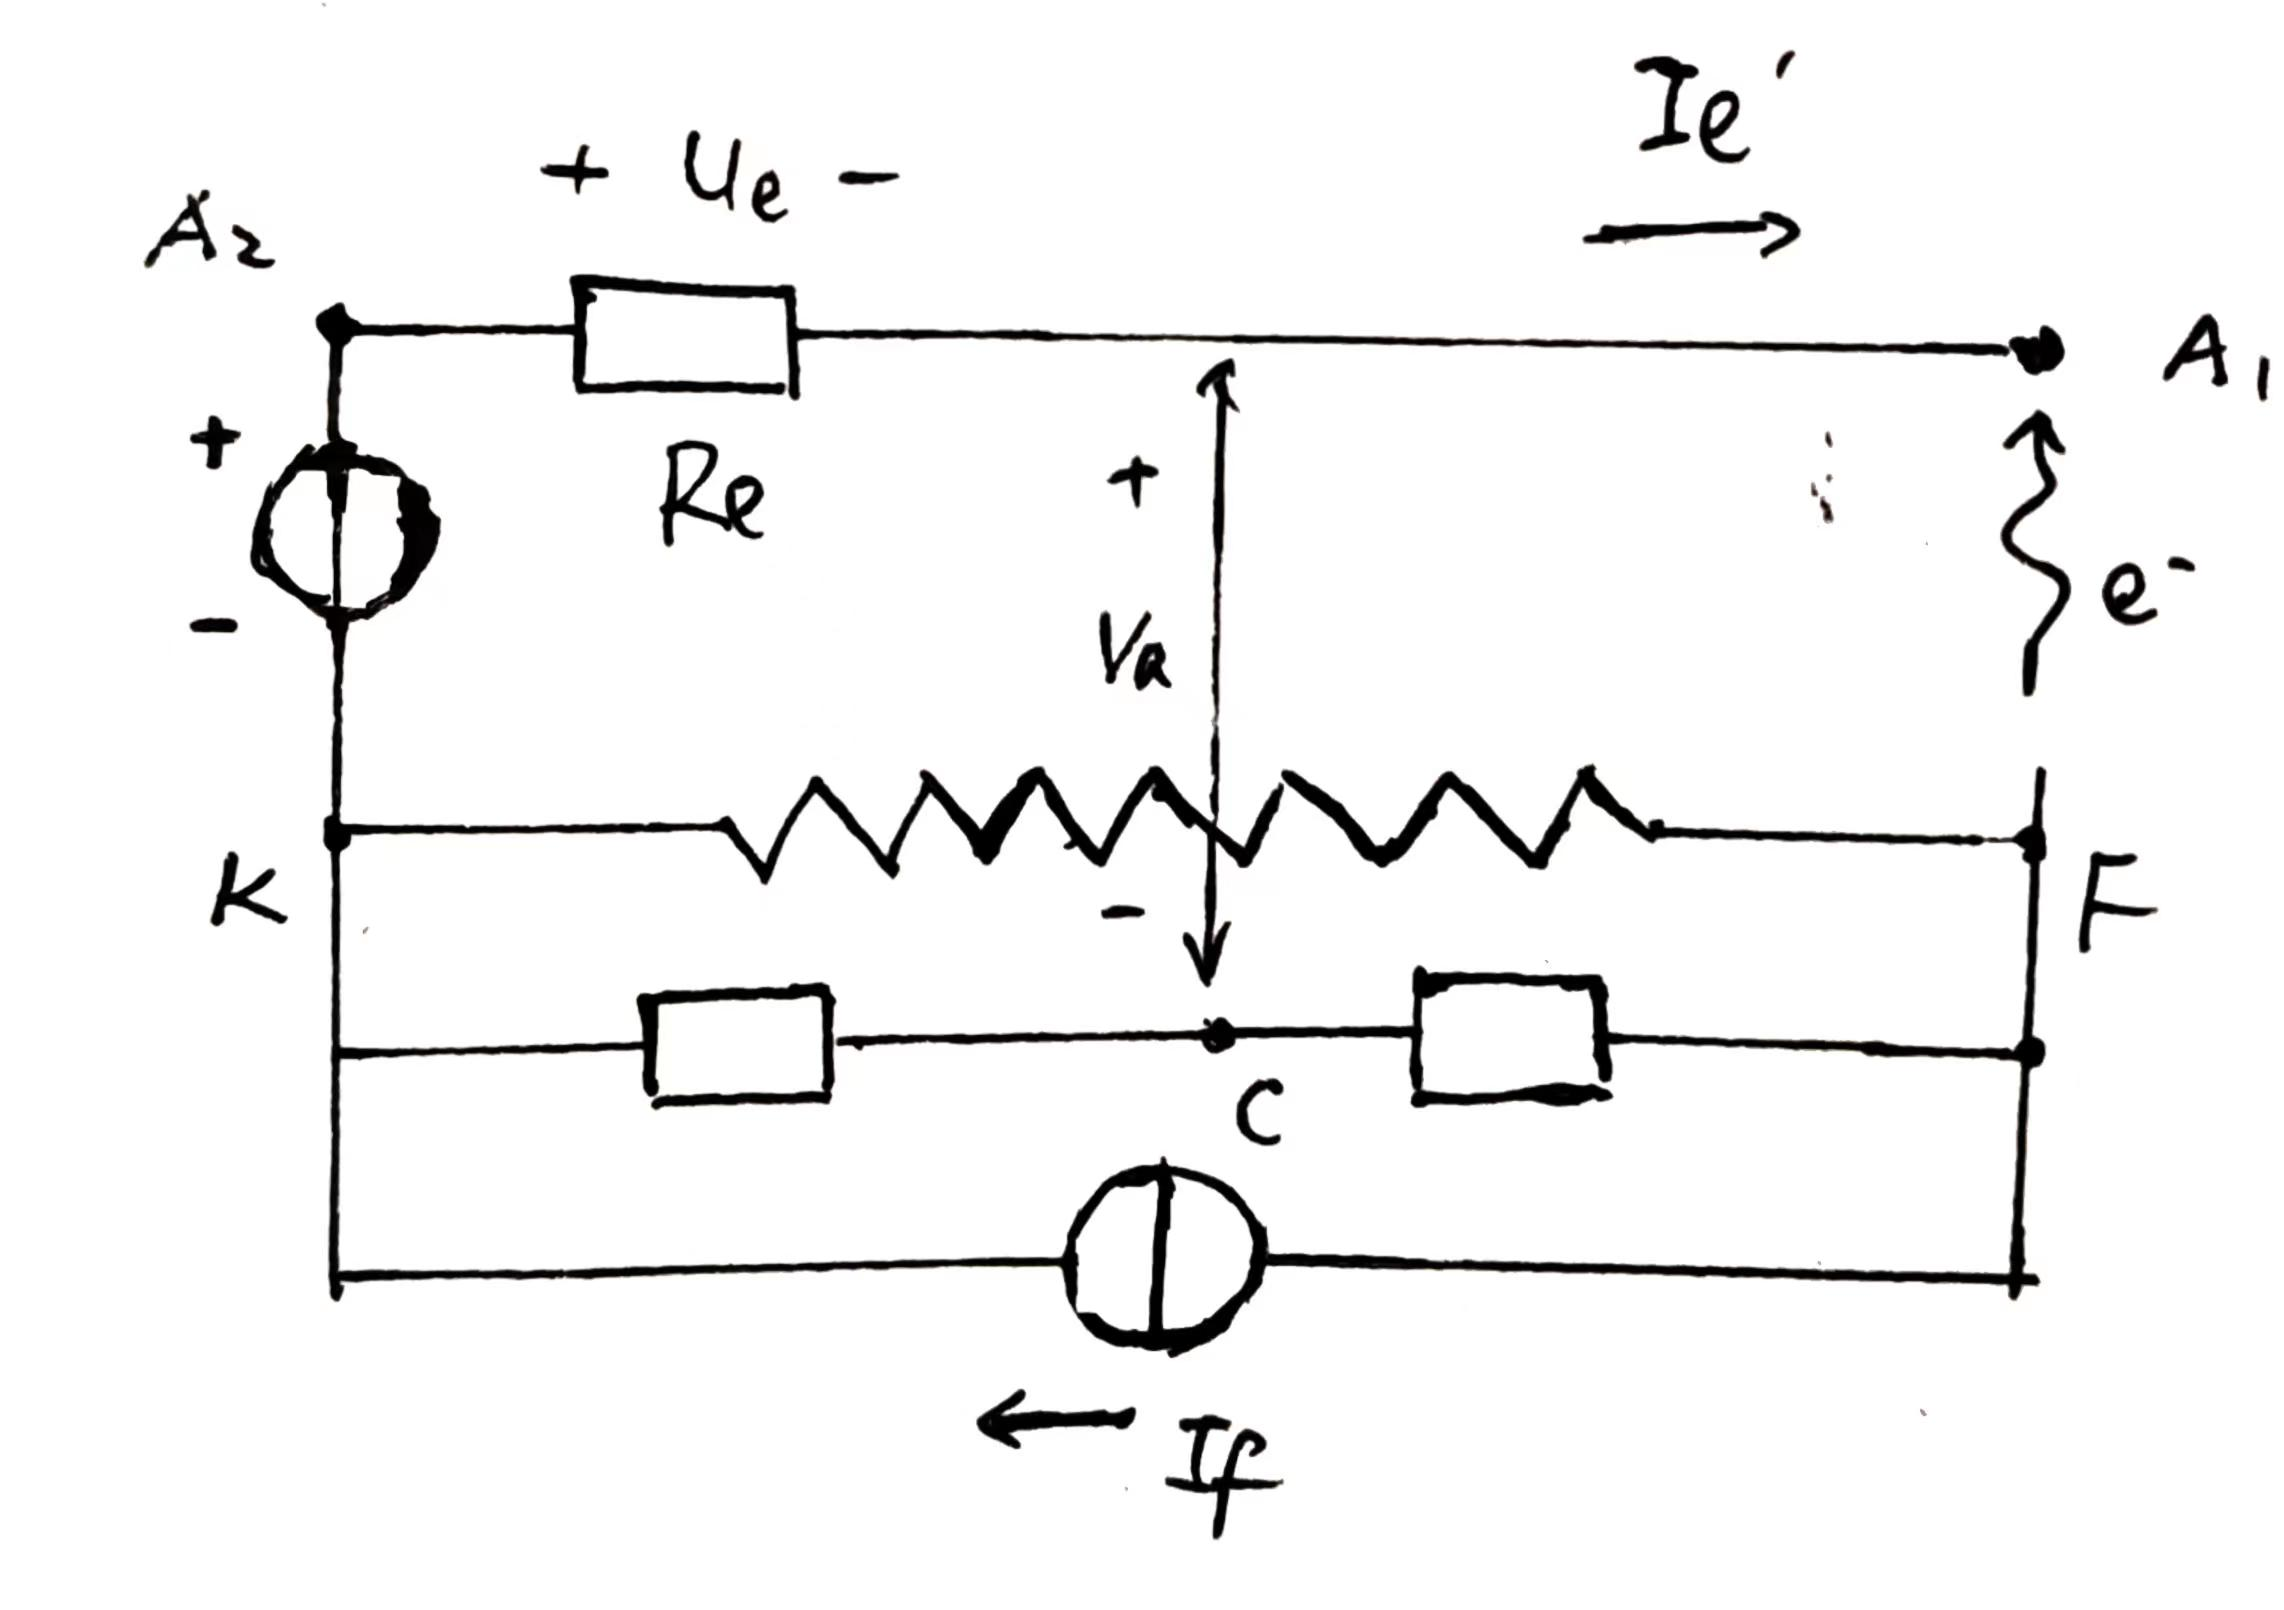
\includegraphics[width=0.9\linewidth]{circuit-design.png}
        \caption{电路设计}
        \label{fg:circuit}
    \end{minipage}
    \begin{minipage}[t]{0.55\linewidth}
        \centering
        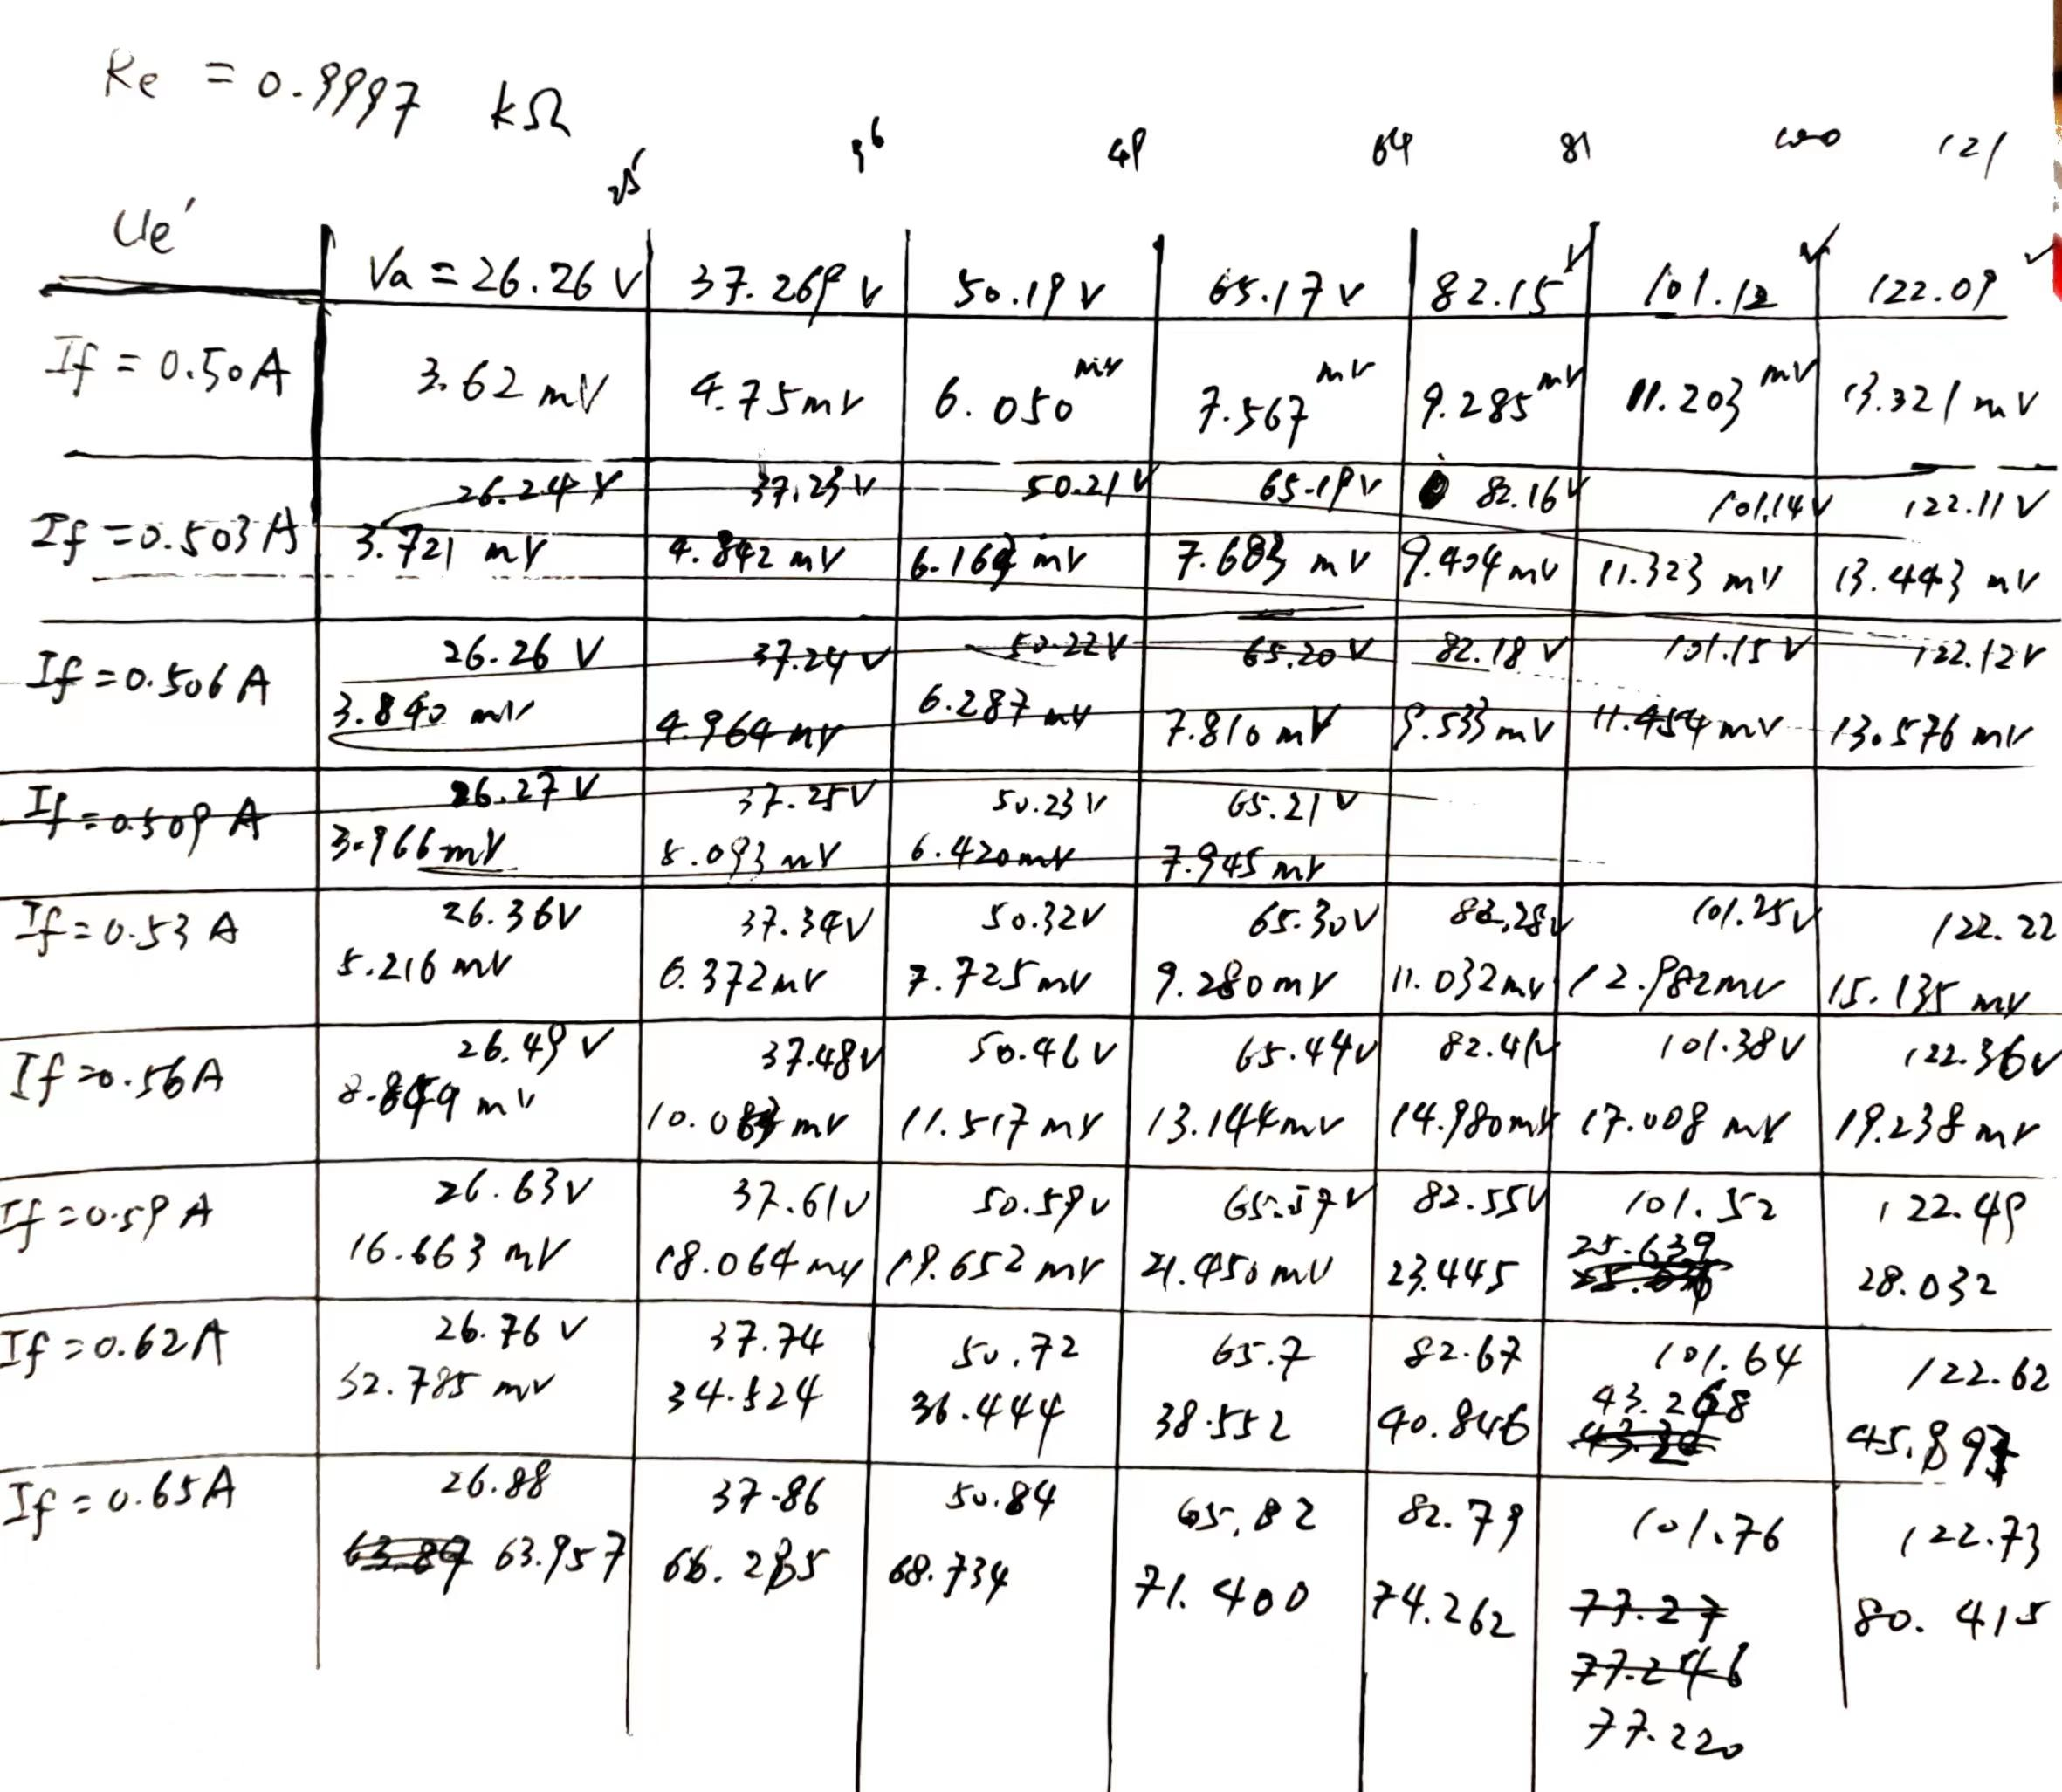
\includegraphics[width=0.9\linewidth]{data.png}
        \caption{原始数据记录}
        \label{fg:data}
    \end{minipage}
\end{figure}
\end{document}